\documentclass[12pt]{article}
% Préambule commun à tous les documents extraits de « La Revue CAPES »
\usepackage[T1]{fontenc}
\usepackage[utf8]{inputenc}
\usepackage{lmodern}
\usepackage{amsmath,amssymb,amsthm,amsfonts,mathrsfs}
\usepackage{setspace}
\usepackage{listings}
\usepackage{pgfplots}
\pgfplotsset{compat=1.18}
\usepackage{longtable}
\usepackage{adjustbox}
\usepackage{lettrine}
\usepackage{tkz-tab}
\usepackage{changepage}
\usepackage{pdflscape}
\usepackage{graphicx}
\usepackage{tikz}
\usepackage{xcolor}
\usepackage[a4paper,top=2cm,bottom=2.5cm,left=2.5cm,right=2cm]{geometry}
\usepackage{fancyhdr}
\usepackage{draftwatermark}
\SetWatermarkText{La RevueCapes}
\SetWatermarkLightness{0.9}
\SetWatermarkScale{2}
\usepackage{hyperref}
\hypersetup{colorlinks=true,linkcolor=blue!50!black,urlcolor=blue!50!black}

\definecolor{revue}{RGB}{20,60,120}

\pagestyle{fancy}
\fancyhf{}
\renewcommand{\headrulewidth}{0.4pt}
\setlength{\headheight}{15pt}

% \entete{Matière}{Titre}{Type de document}
\newcommand{\entete}[3]{%
  \fancyhead[L]{\small\textsc{La Revue CAPES} -- #1}%
  \fancyhead[R]{\small #2}%
  \fancyfoot[C]{\thepage}%
  \thispagestyle{plain}%
  \begin{center}
    {\color{revue}\rule{\textwidth}{1.2pt}}\\[4pt]
    {\small\textsc{Concours directs CAP-CEG / CAPES -- Burkina Faso}}\\[6pt]
    {\LARGE\bfseries\color{revue} #2}\\[6pt]
    {\large\itshape #1 -- #3}\\[2pt]
    {\color{revue}\rule{\textwidth}{1.2pt}}
  \end{center}
  \vspace{0.5cm}%
}

% Encadré pour les remarques ajoutées dans les corrigés
\newcommand{\remarque}[1]{\par\medskip\noindent\fcolorbox{revue}{revue!6}{\parbox{\dimexpr\linewidth-2\fboxsep-2\fboxrule}{\textbf{\color{revue}Remarque.} #1}}\par\medskip}


\begin{document}
\entete{Mathématiques}{Corrigé détaillé du sujet type n°8}{Correction}
\begin{spacing}{1.5}

\textbf{Exercice 1}

1.a) Soit $\overrightarrow{U}=(x,y,z)^T\in \mathbb{R}^3$. On a :

$T(\overrightarrow{U})=T(xe_1+ye_2+ze_3)=xe_3+y(-e_1+e_2+e_3)+ze_3=-ye_1+ye_2+(x+y+z)e_3$.

Ainsi, 

$\overrightarrow{U}=\begin{pmatrix}
x\\
y\\
z\\
\end{pmatrix}\in Ker(T)\Longleftrightarrow \begin{cases}
y=0\\
x+y+z=0
\end{cases}\Longleftrightarrow \begin{cases}
x=k_1, k_1\in \mathbb{R}\\
y=0\\
z=-k_1
\end{cases}\Longleftrightarrow \overrightarrow{U}=k_1\begin{pmatrix}
1\\
0\\
-1
\end{pmatrix}, k_1\in \mathbb{R}$ et $Ker(T)=Vect\langle \begin{pmatrix}
1\\
0\\
-1
\end{pmatrix}\rangle$.


b)  Pour écrire la matrice de l'application linéaire $T$ dans la base $B$ on calcul $T(e_1),
 T(e_2)$ et $T(e_3)$ que l'on exprime dans la base $B$ puis on concatène ces vecteurs pour former $A$.Les vecteurs $T(e_i),(i=1,2,3)$ étant donnés dans l'énoncé on a directement :
 
 $A=\begin{pmatrix}
 0 & -1 & 0 \\ 
 0 & 1 & 0 \\ 
 1 & 1 & 1.
 \end{pmatrix}$
 
 2.a) On a 
 $
 \begin{cases}
 f_1=e_1-e_3\\
 f_2=e_1-e_2\\
 f_3=-e_1+e_2+e_3
 \end{cases}\Leftrightarrow \begin{cases}
 e_3=e_1-f_1=f_2+f_3\\
 e_1=f_2+e_2=f_1+f_2+f_3\\
 e_2=f_1+f_3 (L_3\longleftarrow L3+L1)
 \end{cases}
 $
 
 Ainsi $\mathbb{R}^3=Vect\langle e_1,e_2,e_3\rangle\subset Vect\langle f_1,f_2,f_3\rangle$. La famille $(f_1,f_2,f_3)$ est donc génératrice minimale et c'est une base.
 
 b) On a :
 
 $
 T(f_1)=\begin{pmatrix}
 0 & -1 & 0 \\ 
 0 & 1 & 0 \\ 
 1 & 1 & 1.
 \end{pmatrix}\begin{pmatrix}
1\\
0\\
-1
\end{pmatrix}=0_{\mathbb{R}^3}
$ en remarquant que $f_1\in Ker(T)$

$
T(f_2)=\begin{pmatrix}
 0 & -1 & 0 \\ 
 0 & 1 & 0 \\ 
 1 & 1 & 1.
 \end{pmatrix}\begin{pmatrix}
1\\
-1\\
0
\end{pmatrix}=\begin{pmatrix}
1\\
-1\\
0
\end{pmatrix}=f_2,
$

$
T(f_3)=\begin{pmatrix}
 0 & -1 & 0 \\ 
 0 & 1 & 0 \\ 
 1 & 1 & 1.
 \end{pmatrix}\begin{pmatrix}
-1\\
1\\
1
\end{pmatrix}=\begin{pmatrix}
-1\\
1\\
1
\end{pmatrix}=f_3
$

Ainsi la matrice $B$ de $T$ dans la base $(f_1,f_2,f_3)$ est donnée par :

$
B=\begin{pmatrix}
 0 & 0 & 0 \\ 
 0 & 1 & 0 \\ 
 0 & 0 & 1.
 \end{pmatrix}
 $
 
 3. On va vérifier que $P$ est inversible et calculer $P^{-1}$ en même temps. $P$ est inversible si et seulement si,pour tout $Y\in \mathbb{R}^3$, il existe un unique $X\in \mathbb{R}^3$ tel que $PX=Y$. On fixe donc $Y=(y_1,y_2,y_3)^T\in \mathbb{R}^3$ et on résout le système : 
 
 $
 \begin{cases}
 x_1+x_2-x_3=y_1\\
 -x_2+x_3=y_2\\
 -x_1+x_3=y_3
 \end{cases}\Leftrightarrow \begin{cases}
 x_2=y_1+y_3 (L_1\longleftarrow L_1+L3)\\
 x_3=y_1+y_2+y_3\\
 x_1=y_1+y_2
 \end{cases}
 $
 
  Le système précédent admet donc une unique solution,$P$ est inversible et $P^{-1}$ est donnée par :
  
  $
  \begin{pmatrix}
 1 & 1 & 0 \\ 
 1 & 0 & 1 \\ 
 1 & 1 & 1.
 \end{pmatrix} \hspace*{1cm}\begin{cases}
 x_1=\textbf{1} y_1+\textbf{1}y_2+\textbf{0}y_3\\
 x_2=\textbf{1} y_1+\textbf{0}y_2+\textbf{1}y_3\\
 x_3=\textbf{1} y_1+\textbf{1}y_2+\textbf{1}y_3
 \end{cases}
 $
 
  \textbf{Deuxième méthode} : $P$ est la matrice de passage de la base $B$ à la base $V$, elle est
 donc inversible. La matrice $P^{-1}$ est la matrice de passage de la base $V$ à la base $B$. Pour
 écrire cette matrice on utilise la relation (obtenue précédemment dans l'exercice) :
 
 $
 \begin{cases}
 e_1=f_1+f_2+y_3\\
 e_2=f_1+f_3\\
 e_3=f_2+f_3
\end{cases}
 $
 
 Cela nous donne directement $P^{-1}$ en concaténant les $e_i$ exprimés en fonction des $f_i$.
Finalement la formule du changement de base sur les matrices donne:

$
A=PBP^{-1}
$

\underline{\textbf{Rappel :}}

 Soit $f :E\rightarrow E$ une application linéaire. Soit $B$ et $B'$ deux bases de $E$. On note $A$
 (respectivement $B$) la matrice de $f$ dans la base $B$ (respectivement $B'$). Soit $u$ un vecteur
 de $E$. Soit $X$ le vecteur colonne associé à $u$ dans la base $B$  et $Y$ le vecteur colonne associé
 à $u$ dans la base $B'$. On a la relation $X=PY$ avec $P$ la matrice de passage de $B$ à $B'$.
 
 Si on calcul $f(u)$ et que l'on exprime le résultat dans la base $B$ on a:
 
$ [f(u)]_B=AX$

 Calculons maintenant $f(u)$ en passant par la base $B'$. On a
$ [f(u)]_{B^{'}}=BY$
 
  On passe d'une expression à l'autre en utilisant la matrice de passage $P$ donc:

$ [f(u)]_B=P[f(u)]_{B^{'}}$

Soit $AX=PBY$, mais $Y=P^{-1}X$ donc finalement : 

$AX=PBP^{-1}X$.

Cette relation implique donc l'égalité matricielle $A=PBP^{-1}$.






\medskip\textbf{Exercice 2} 

Le plan $(P)$ est rapporté à un repère orthonormé direct $(\overrightarrow{0} ; \overrightarrow{u}; \overrightarrow{v})$. On désigne par \(T\) l'application de \((P)\) dans \((P)\) qui, à tout point \(M\) d'affixe \(z\), associe le point \(M'\) d'affixe : 
\[
z' = (1+i)z - i.
\]

\medskip
\textbf{1. Décomposition de \(T\) en une rotation et une homothétie}

\begin{itemize}
    \item On écrit \(z' = (1+i)z - i = \sqrt{2}e^{i\pi/4}z - i\).
    \item L'application \(T\) est donc une homothétie de rapport \(k = |1+i| = \sqrt{2}\) suivie d'une rotation d'angle \(\theta = \frac{\pi}{4}\), le tout combiné avec une translation de vecteur \(-i\).
    \item Le point invariant par \(T\) (point fixe) est obtenu en résolvant \(z' = z\), soit :
    \[
    z = \sqrt{2}e^{i\pi/4}z - i \implies z(1 - \sqrt{2}e^{i\pi/4}) = -i \implies z = \frac{-i}{1 - \sqrt{2}e^{i\pi/4}}.
    \]
    \item Simplifions : \(z = \Omega = \frac{-i(1 - \sqrt{2}e^{-i\pi/4})}{(1 - \sqrt{2}e^{i\pi/4})(1 - \sqrt{2}e^{-i\pi/4})} = -1 - i\).
    \item Le point invariant \(\Omega\) a donc pour affixe \(z_\Omega = -1 - i\).
    \item L'angle orienté \((\overrightarrow{\Omega M}, \overrightarrow{MM'})\), pour \(M \neq \Omega\), est \(\theta = \frac{\pi}{4}\).
\end{itemize}

\medskip
\textbf{2.a) Construction de \(M'\), image de \(M\) par \(T\)}

Soit \(M\) un point donné d'affixe \(z\), l'affixe de \(M'\) est :
\[
z' = \sqrt{2}e^{i\pi/4}z - i.
\]
Pour tracer \(M'\), on applique successivement :
\begin{itemize}
    \item une homothétie de rapport \(\sqrt{2}\),
    \item une rotation d'angle \(\frac{\pi}{4}\),
    \item une translation de vecteur \(-i\).
\end{itemize}

\textbf{2.b) Image de la droite \((D)\) par \(T\)}

La droite \((D)\) a pour équation \(y = x\), soit \(z = x + ix\). On a donc :
\[
z' = (1+i)z - i = (1+i)(x + ix) - i = (1 - x) + i(2x - 1).
\]
Les affixes \(z'\) des points de \((D')\) satisfont l'équation :
\[
x' = 1 - y', \quad \text{soit } y' = -x' + 1.
\]
La droite \((D')\) a donc pour équation \(y = -x + 1\).

\medskip
\textbf{3.a) Existence et unicité de \(B\)}

On cherche un point \(B\) distinct de \(\Omega\) tel que \(z_0z'_0 = 1\), avec \(z'_0 = (1+i)z_0 - i\). On a donc :
\[
z_0 \big((1+i)z_0 - i\big) = 1 \implies z_0^2(1+i) - iz_0 - 1 = 0.
\]
Posons \(z_0 = x + iy\) (où \(x, y \in \mathbb{R}\)) et résolvons cette équation complexe pour trouver \(z_0\). 

Le calcul donne \(z_0 = \frac{1 + i}{2}\). Le point \(B'\), image de \(B\), est alors \(z'_0 = \frac{2}{1+i} = 1 - i\).

\medskip
3.b) Cocyclicité des points \(\Omega', \Omega, B, B'\)

Le point \(\Omega'\), symétrique de \(\Omega\) par rapport à \(O\), a pour affixe \(z_{\Omega'} = 1 + i\).

Les points \(\Omega', \Omega, B, B'\) sont cocycliques si leurs affixes satisfont la relation de cercle. On montre que le centre \(G\) de ce cercle a pour affixe :
\[
z_G = \frac{z_\Omega + z_{\Omega'} + z_B + z_{B'}}{4} = \frac{(-1-i) + (1+i) + \frac{1+i}{2} + (1-i)}{4}.
\]
Le calcul donne \(z_G = \frac{1}{2}\).

Ainsi, le centre du cercle est \(G\) d'affixe \(z_G = \frac{1}{2}\).









\begin{center}
\textbf{Constructions Géométriques}


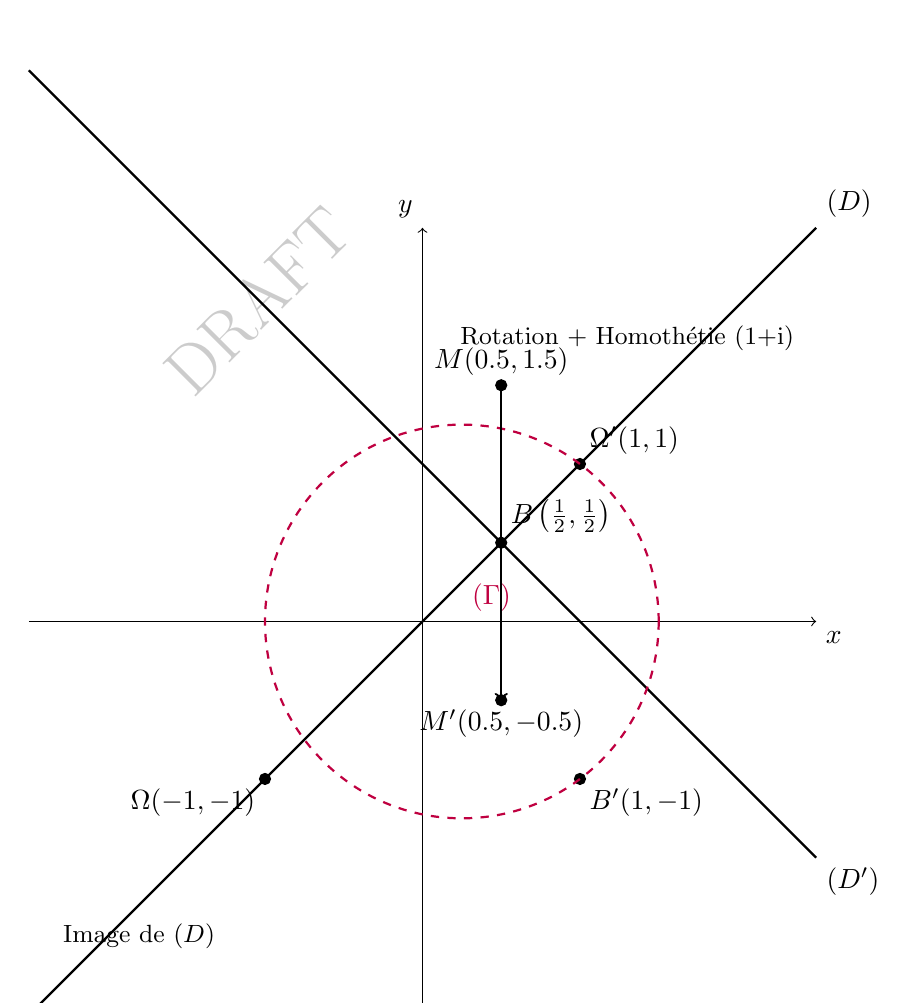
\begin{tikzpicture}[scale=2]
    % Repère orthonormé
    \draw[->] (-2.5, 0) -- (2.5, 0) node[anchor=north west] {$x$};
    \draw[->] (0, -2.5) -- (0, 2.5) node[anchor=south east] {$y$};
    \draw[thick] (-2.5, -2.5) -- (2.5, 2.5) node[above right] {$(D)$};
    \draw[thick, black] (-2.5, 3.5) -- (2.5, -1.5) node[below right] {$(D')$};
    
    % Points principaux
    \filldraw[black] (-1,-1) circle (1pt) node[below left] {$\Omega(-1, -1)$};
    \filldraw[black] (1,1) circle (1pt) node[above right] {$\Omega'(1, 1)$};
    \filldraw[black] (0.5, 0.5) circle (1pt) node[above right] {$B\left(\frac{1}{2}, \frac{1}{2}\right)$};
    \filldraw[black] (1,-1) circle (1pt) node[below right] {$B'(1, -1)$};
    
    % Cercle passant par Omega, Omega', B et B'
    \draw[thick, dashed, purple] (0.25,0) circle (1.25) node[above right] {$(\Gamma)$};
    
    % Exemple point M et son image M'
    \filldraw[black] (0.5, 1.5) circle (1pt) node[above] {$M(0.5, 1.5)$};
    \filldraw[black] (0.5, -0.5) circle (1pt) node[below] {$M'(0.5, -0.5)$};
    \draw[->, thick, black] (0.5, 1.5) -- (0.5, -0.5);

    % Légendes et étiquettes
    \node at (1.3, 1.8) [black] {\small Rotation + Homothétie (1+i)};
    \node at (-1.8, -2) [black] {\small Image de $(D)$};
\end{tikzpicture}
\end{center}

\quad



\medskip\textbf{Exercice 3}


1. Calculons

$I=\int\int_D\frac{dxdy}{(1+x^2+y^2)^2}$ ou $D=\lbrace {(x,y) \in \mathbb{R}^2,\vert x\vert \leq x^2+y^2\leq 1\rbrace}$.

Passage aux coordonnées polaires :

Soit $x=r\cos \theta$ et $y=r\sin\theta$

$x^2+y^2=r^2$

$x^2+y^2\leq 1\Rightarrow r^2\leq 1\Rightarrow 0\leq r\leq 1$

$\vert x\vert \leq x^2+y^2\Rightarrow \theta\in [0,2\pi]$

A travers le jacobien, $dxdy=rdrd\theta$

Donc,

$I=\int_0^1\int_0^{2\pi}\frac{rdrd\theta}{(1+r^2)^2}=\int_0^{2\pi}d\theta\times\int_0^1\frac{rdr}{(1+r^2)^2}=2\pi\int_0^1\frac{rdr}{(1+r^2)^2}$

Posons $u=1+r^2$, $du=2rdr\Longrightarrow dr=\frac{du}{2r}$

Si $r\to 0$, $u\to 1$ et si  $r\to 1$, $u\to 2$

L'intégrale devient :

$I=2\pi\times\frac{1}{2}\int_1^2\frac{du}{u^2}=\pi[-\frac{1}{u}]_1^2=\pi(-\frac{1}{2}+1)=\frac{\pi}{2}$


2. Calculons l'intégrale double

$J=\int\int_D(x+y)^2dxdy$ ou $D=\lbrace (x,y)\in \mathbb{R}^2, x^2+y^2-x \leq 0;x^2+y^2-y \geq 0$ et $y \geq 0 \rbrace$.

 Définition et analyse de la région \(D\)
 
La région \(D\) est définie par trois inégalités :
\begin{itemize}
    \item \( x^2 + y^2 - x \leq 0 \), ce qui correspond au disque de centre \(\left( \frac{1}{2}, 0 \right)\) et de rayon \(\frac{1}{2}\).
    \item \( x^2 + y^2 - y \geq 0 \), ce qui correspond à l'extérieur du disque de centre \((0, \frac{1}{2})\) et de rayon \(\frac{1}{2}\).
    \item \( y \geq 0 \), restreignant la région au demi-plan supérieur.
\end{itemize}

\textbf{Intersection :} La région \(D\) est l'intersection du disque centré en \(\left( \frac{1}{2}, 0 \right)\) avec l'extérieur du disque centré en \((0, \frac{1}{2})\), dans le demi-plan supérieur. Les frontières des disques peuvent être exprimées en coordonnées polaires :
\begin{itemize}
    \item \( (x - \frac{1}{2})^2 + y^2 = \frac{1}{4} \Rightarrow r = \cos\theta \),
    \item \( x^2 + (y - \frac{1}{2})^2 = \frac{1}{4} \Rightarrow r = \sin\theta \).
\end{itemize}
La région \(D\) en polaires est donc donnée par :
\[ \theta \in [0, \frac{\pi}{2}], \quad r \in [\sin\theta, \cos\theta]. \]

 Réécriture de l'intégrale en coordonnées polaires
 
En polaires :

\begin{align*}
    x &= r\cos\theta, \quad y = r\sin\theta, \quad x + y = r(\cos\theta + \sin\theta), \\
    dxdy &= r drd\theta.
\end{align*}
L'intégrale devient :
\[
    J = \int_0^{\pi/2} \int_{\sin\theta}^{\cos\theta} \left[r(\cos\theta + \sin\theta)\right]^2 r \, dr \, d\theta.
\]

Développons \((\cos\theta + \sin\theta)^2\) :
\[
    (\cos\theta + \sin\theta)^2 = \cos^2\theta + 2\cos\theta\sin\theta + \sin^2\theta = 1 + 2\cos\theta\sin\theta.
\]
Ainsi :
\[
    J = \int_0^{\pi/2} \int_{\sin\theta}^{\cos\theta} r^3 \left(1 + 2\cos\theta\sin\theta\right) \, dr \, d\theta.
\]

\textbf{Calcul de l'intégrale}

 Intégration par rapport à \(r\)
 
\[
    \int_{\sin\theta}^{\cos\theta} r^3 \, dr = \left[ \frac{r^4}{4} \right]_{\sin\theta}^{\cos\theta} = \frac{\cos^4\theta}{4} - \frac{\sin^4\theta}{4}.
\]
Substituons dans \(J\) :
\[
    J = \int_0^{\pi/2} \left[ \frac{\cos^4\theta}{4} - \frac{\sin^4\theta}{4} \right] \left(1 + 2\cos\theta\sin\theta\right) d\theta.
\]

 Séparation des termes
 
Développons :
\begin{align*}
    J &= \frac{1}{4} \int_0^{\pi/2} \cos^4\theta (1 + 2\cos\theta\sin\theta) \, d\theta - \frac{1}{4} \int_0^{\pi/2} \sin^4\theta (1 + 2\cos\theta\sin\theta) \, d\theta. \\
    &= \frac{1}{4} \left[ \int_0^{\pi/2} \cos^4\theta \, d\theta + 2 \int_0^{\pi/2} \cos^5\theta\sin\theta \, d\theta \right] \\
    &\quad - \frac{1}{4} \left[ \int_0^{\pi/2} \sin^4\theta \, d\theta + 2 \int_0^{\pi/2} \cos\theta\sin^5\theta \, d\theta \right].
\end{align*}

 Calcul des intégrales élémentaires
 
 \(\int_0^{\pi/2} \cos^4\theta \, d\theta\) et \(\int_0^{\pi/2} \sin^4\theta \, d\theta\) : Utilisons les formules de réduction :
\[
    \int_0^{\pi/2} \cos^4\theta \, d\theta = \int_0^{\pi/2} \sin^4\theta \, d\theta = \frac{3\pi}{16}.
\]

 \(\int_0^{\pi/2} \cos^5\theta\sin\theta \, d\theta\) et \(\int_0^{\pi/2} \cos\theta\sin^5\theta \, d\theta\) : Par substitution \(u = \cos\theta\) ou \(u = \sin\theta\), on trouve :
\[
    \int_0^{\pi/2} \cos^5\theta\sin\theta \, d\theta = \int_0^{\pi/2} \cos\theta\sin^5\theta \, d\theta = \frac{1}{6}.
\]

Résultat final

En combinant tous les termes :
\[
    J = \frac{1}{4} \left[ \frac{3\pi}{16} + 2 \cdot \frac{1}{6} \right] - \frac{1}{4} \left[ \frac{3\pi}{16} + 2 \cdot \frac{1}{6} \right] = \frac{1}{15}.
\]

\textbf{Ainsi, la valeur de l'intégrale est :}
\[
    J = \frac{1}{15}.
\]




3. Soit $D=\lbrace (x,y,z)\in \mathbb{R}^3;x\geq 0,y\geq 0,z\geq 0,x+y+z\leq 1 \rbrace$.

Utilisons le changement de variable $u=x+y+z; v=\frac{z}{y+z}; w=\frac{y+z}{x+y+z}$ pour calculer

$S=\int\int_D\frac{z^3}{(x+y+z)(y+z)}dxdydz$.

On effectue le changement de variables suivant :
\[
u = x + y + z, \quad v = \frac{z}{y + z}, \quad w = \frac{y + z}{x + y + z}.
\]

 Jacobien du changement de variables

Pour déterminer le jacobien de ce changement de variables, nous devons calculer le déterminant de la matrice des dérivées partielles des nouvelles variables \( u, v, w \) par rapport aux anciennes variables \( x, y, z \). Le jacobien \( J \) est donné par :
\[
J = \det \begin{pmatrix} 
\frac{\partial u}{\partial x} & \frac{\partial u}{\partial y} & \frac{\partial u}{\partial z} \\
\frac{\partial v}{\partial x} & \frac{\partial v}{\partial y} & \frac{\partial v}{\partial z} \\
\frac{\partial w}{\partial x} & \frac{\partial w}{\partial y} & \frac{\partial w}{\partial z}
\end{pmatrix}.
\]

Cela peut être calculé en effectuant les dérivées partielles de chaque variable par rapport à \( x \), \( y \), et \( z \), et en déterminant le déterminant de la matrice résultante.

 L'intégrale après changement de variables

L'intégrale que nous devons calculer est :
\[
S = \int \int \int_D \frac{z^3}{(x + y + z)(y + z)} \, dx \, dy \, dz.
\]

Après le changement de variables, l'intégrale devient :
\[
S = \int_0^1 \int_0^1 \int_0^1 \frac{u^3 v^3}{u^3 v} \cdot J \, du \, dv \, dw,
\]
où \( J \) est le jacobien du changement de variables.

 Simplification de l'intégrale

Simplifions l'expression de l'intégrale :
\[
S = \int_0^1 \int_0^1 \int_0^1 u^2 v^2 \, du \, dv \, dw.
\]

Cela donne une intégrale séparée, et les intégrales sur \( u \), \( v \), et \( w \) peuvent être calculées indépendamment :
\[
\int_0^1 u^2 \, du = \frac{1}{3}, \quad \int_0^1 v^2 \, dv = \frac{1}{3}, \quad \int_0^1 1 \, dw = 1.
\]

 Conclusion

En multipliant ces résultats, nous obtenons :
\[
S = \frac{1}{3} \cdot \frac{1}{3} \cdot 1 = \frac{1}{9}.
\]

Ainsi, l'intégrale \( S \) est égale à \( \frac{1}{9} \)


4. Calculons l'aire du domaine elliptique :

$E = \lbrace (x,y)\in \mathbb{R}^2;\frac{x^2}{a^2}+\frac{y^2}{b^2}\leq 1\rbrace$.

Il s'agit d'une ellipse centrée en \( (0, 0) \), avec des axes de longueurs \( 2a \) et \( 2b \) dans les directions \( x \) et \( y \), respectivement.

 Changement de variables

Pour calculer l'aire de l'ellipse, nous utilisons un changement de variables pour transformer l'ellipse en un cercle unité. On définit les nouvelles variables \( u \) et \( v \) par :
\[
u = \frac{x}{a}, \quad v = \frac{y}{b}.
\]

Ainsi, l'ellipse devient l'ensemble des points \( (u, v) \) satisfaisant :
\[
u^2 + v^2 \leq 1,
\]
c'est-à-dire un disque de rayon 1 centré en \( (0, 0) \).

Jacobien du changement de variables

Le jacobien du changement de variables \( (x, y) \mapsto (u, v) \) est donné par le déterminant de la matrice des dérivées partielles :
\[
J = \det \begin{pmatrix} \frac{\partial u}{\partial x} & \frac{\partial u}{\partial y} \\ \frac{\partial v}{\partial x} & \frac{\partial v}{\partial y} \end{pmatrix}
= \det \begin{pmatrix} \frac{1}{a} & 0 \\ 0 & \frac{1}{b} \end{pmatrix}
= \frac{1}{ab}.
\]

Le facteur de transformation de l'aire est donc \( \frac{1}{ab} \).

 Aire du domaine elliptique

L'aire du domaine \( E \) dans le plan \( (x, y) \) est égale à l'aire du disque unité dans le plan \( (u, v) \) multipliée par le facteur de transformation \( \frac{1}{ab} \). L'aire du disque unité est \( \pi \), donc l'aire de \( E \) est :
\[
\text{Aire}(E) = \pi \cdot a \cdot b.
\]

Conclusion

L'aire du domaine elliptique \( E \) est donnée par :
\[
\text{Aire}(E) = \pi \cdot a \cdot b.
\]





\medskip\textbf{Exercice 4}


On pose $f(n)=\int_{0}^{1}x^ne^{-x}dx$  $\forall n\in \mathbb{N}$.

1. Montrons que la suite $(f(n))$ est positive et décroissante.

$\forall x\in [0,1]$, $x^ne^{-x}>0$ donc $\int_{0}^{1}x^ne^{-x}dx>0$ d'où $f(n)>0$.

$\forall x\in [0,1]$, $0\leq x\leq 1\Rightarrow 0\leq x^{n+1}\leq x^n$

Donc $\int_{0}^{1}x^{n+1}e^{-x}dx\leq \int_{0}^{1}x^ne^{-x}dx$. Autrement dit $f(n+1)\leq f(n)$, ainsi cette suite est décroissante.

\medskip
Donnons une relation de récurrence entre $f(n)$ et $f(n-1)$.
 
 $f(n)=\int_{0}^{1}x^ne^{-x}dx$
 
 Posons 
 

$ u =x^n\longrightarrow u'=nx^{n-1}\\
 v' =e^{-x}\longrightarrow v=-e^{-x}
$ 
 
 $\Rightarrow f(n)=[-x^ne^{-x}]_0^1+\int_{0}^{1}nx^{n-1}e^{-x}dx$ avec $[-x^ne^{-x}]_0^1=-e^{-1}=-\frac{1}{e}$ et $\int_{0}^{1}nx^{n-1}e^{-x}dx=nf(n-1)$
 
 $\Rightarrow f(n)=-\frac{1}{e}+nf(n-1)$.
 
 
 2. Montrons par récurrence que pour tout $n\in \mathbb{N}$, $f(n)= \frac{n!}{e}(e-\sum_{k=0}^{n}\frac{1}{k!})$
 
 Pour $n=0$, $\int_{0}^{1}x^{0}e^{-x}dx=[-e^{-x}]_0^1=-\frac{1}{e}+1$
 
 On a : $\frac{0!}{e}(e-\sum_{k=0}^{0}\frac{1}{k!})=\frac{1}{e}(e-1)=1-\frac{1}{e}$
 
 Les deux sont égaux, alors l'hypothèse est vérifié au rang 0.
 
 Supposons l'hypothèse vrai à l'ordre $n-1$,c'est-à-dire $f(n-1)= \frac{(n-1)!}{e}(e-\sum_{k=0}^{n-1}\frac{1}{k!})$ et vérifions au rang $n$.
 
 \begin{align*}
f(n) &= -\frac{1}{e} + n f(n-1) \\
     &= -\frac{1}{e} + n \frac{(n-1)!}{e} \left( e - \sum_{k=0}^{n-1} \frac{1}{k!} \right) \\
     \text{avec } n(n-1)! = n! \\
     &= -\frac{1}{e} + \frac{n!}{e} \left( e - \sum_{k=0}^{n-1} \frac{1}{k!} \right) \\
     &= -\frac{n!}{n!e} + \frac{n!}{e} \left( e - \sum_{k=0}^{n-1} \frac{1}{k!} \right) \\
     &= \frac{n!}{e} \left( -\frac{1}{n!} + e - \sum_{k=0}^{n-1} \frac{1}{k!} \right) \\
     \text{avec } -\frac{1}{n!} - \sum_{k=0}^{n-1} \frac{1}{k!} &= -\sum_{k=0}^{n} \frac{1}{k!} \\
f(n) &= \frac{n!}{e} \left( e - \sum_{k=0}^{n} \frac{1}{k!} \right)
\end{align*}

 
 L'hypothèse est donc vrai pour tout $n$. Ce qui achève la récurrence.
 
 3. Montrons que l'on a $\frac{1}{e(n+1)}\leq f(n)\leq \frac{1}{n+1}$.
 
 On a :
 

\begin{align*}
0 \leq x \leq 1 &\Rightarrow -1 \leq -x \leq 0 \\
&\Rightarrow e^{-1} \leq e^{-x} \leq e^{0} \\
&\Rightarrow \frac{1}{e} \times x^n \leq x^n e^{-x} \leq x^n \\
&\Rightarrow \frac{1}{e} \int_{0}^{1} x^n \, dx \leq\int_{0}^{1} x^n e^{-x} \, dx \leq \\
\int_{0}^{1} x^n \, dx \\
\text{avec } \int_{0}^{1} x^n e^{-x} \, dx = f(n) \text{ et } \int_{0}^{1} x^n \, dx = \left[ \frac{1}{n+1} x^{n+1} \right]_{0}^{1} = \frac{1}{n+1} \\
&\Rightarrow \frac{1}{e(n+1)} \leq f(n) \leq \frac{1}{n+1}
\end{align*}

 d'où le résultat
 
 4. Déduisons la nature des séries $\sum_{n=1}^{+\infty}f(n)$, $\sum_{n=1}^{+\infty}\frac{f(n)}{n}$ et $\sum_{n=1}^{+\infty}(-1)^nf(n)$.
 
 On a : $\frac{1}{e(n+1)}\leq f(n)\leq \frac{1}{n+1}$
 
 
 \medskip
 $\bullet \sum_{n=1}^{+\infty}f(n)$

$f(n)$ est minorée par $\frac{1}{e(n+1)}\sim \frac{1}{en}$  qui est le terme général d'une série de Riemann divergente donc la série de terme général $f(n)$, c'est-à-dire $\sum_{n=1}^{+\infty}f(n)$ diverge.
 
 \medskip
 $\bullet \sum_{n=1}^{+\infty}\frac{f(n)}{n}$
 
 $\frac{1}{e(n+1)}\leq f(n)\leq \frac{1}{n+1}\Rightarrow \frac{1}{en(n+1)}\leq \frac{f(n)}{n}\leq \frac{1}{n(n+1)}$
 
 $\frac{f(n)}{n}$ est majorée par $\frac{1}{n(n+1)}\sim \frac{1}{n^2}$ qui est le terme générale d'une série de Riemann convergente donc la série de terme général $\frac{f(n)}{n}$ converge.
 
 $\bullet \sum_{n=1}^{+\infty}(-1)^nf(n)$
 
 $f(n)$ est positive et décroissante, donc la série de terme général $(-1)^nf(n)$ est une série alternée convergente.
 
 
 5. Déterminons le rayon de convergence de la série entière $\sum_{n=1}^{+\infty}f(n)x^n$.

 Soit $R$ le rayon de convergence de la série entière. Comme la série de terme général $f(n)$ diverge cela signifie que 1  n'est pas dans le disque de convergence sinon
$\sum_{n=1}^{+\infty}f(n)1^n=\sum_{n=1}^{+\infty}f(n)$ convergerait, cela entraine que $R\geq 1$.

Comme la série de terme général $(-1)^nf(n)$ converge, cela signifie que -1 est dans le disque de 
converge donc $R\leq 1$ , en effet

$\sum_{n=1}^{+\infty}f(n)(-1)^n< +\infty$

Donc $R=1$

\end{spacing}
\end{document}
